
\section{Buffer}

Buffer werden genutzt um Daten von der CPU zur GPU zu bewegen. Aus der Sicht einer Programmiersprache sind Buffer simple Arrays, also ein zusammenhängendes Stück im Speicher.

\subsection{Exkurs Normalized Device Coordinates}
\label{sec:buffer:ndc}
In den folgenden Kapiteln werden die Positionen von Verticies genutzt. Diese Positionen werden in Grafik APIs in einem speziellen Format, den sogenannten Normalized Device Coordinates (NDC) angegeben.

%würfel code von https://tex.stackexchange.com/a/28286
\begin{figure}
    \caption{Ein rechtshändisches Koordinatensystem (OpenGL)}
    \label{fig:coordinatesystemsright}
    \begin{center}
        \begin{tikzpicture}
            \def\size{2}
            \def\cocenterx{3}
            \def\cocentery{0.5}
            \def\cocenterz{0}

            \coordinate (O) at (0,0,0);
            \coordinate (A) at (0,\size,0);
            \coordinate (B) at (0,\size,\size);
            \coordinate (C) at (0,0,\size);
            \coordinate (D) at (\size,0,0);
            \coordinate (E) at (\size,\size,0);
            \coordinate (F) at (\size,\size,\size);
            \coordinate (G) at (\size,0,\size);
            \draw[grey] (O) -- (C) -- (G) -- (D) -- cycle;% Bottom Face
            \draw[grey] (O) -- (A) -- (E) -- (D) -- cycle;% Back Face
            \draw[grey] (O) -- (A) -- (B) -- (C) -- cycle;% Left Face
            \draw       (D) -- (E) -- (F) -- (G) -- cycle;% Right Face
            \draw       (C) -- (B) -- (F) -- (G) -- cycle;% Front Face
            \draw       (A) -- (B) -- (F) -- (E) -- cycle;% Top Face
            
            \node at (O) {\tiny\hspace{-4em}(-1,-1,-1)};
            \node at (A) {\tiny\hspace{-5em}(-1,1,-1)};
            \node at (B) {\tiny\hspace{-5em}(-1,1,1)};
            \node at (C) {\tiny\hspace{-5em}(-1,-1,1)};
            \node at (D) {\tiny\hspace{4em}(1,-1,-1)};
            \node at (E) {\tiny\hspace{4em}(1,1,-1)};
            \node at (F) {\tiny\hspace{5em}(1,1,1)};
            \node at (G) {\tiny\hspace{4.5em}(1,-1,1)};

            \coordinate (CO) at (0+\cocenterx,0+\cocentery,0+\cocenterz);
            \coordinate (CX) at (1+\cocenterx,0+\cocentery,0+\cocenterz);
            \coordinate (CY) at (0+\cocenterx,1+\cocentery,0+\cocenterz);
            \coordinate (CZ) at (0+\cocenterx,0+\cocentery,1+\cocenterz);

            \draw[thick,->] (CO) -- (CX);
            \draw[thick,->] (CO) -- (CY);
            \draw[thick,->] (CO) -- (CZ);

            \node at (CX) {\tiny\hspace{2em}+X};
            \node at (CY) {\tiny\hspace{2em}+Y};
            \node at (CZ) {\tiny\hspace{3em}+Z};
        \end{tikzpicture}
    \end{center}
\end{figure}

\begin{figure}
    \caption{Ein linkshändisches Koordinatensystem (Direct3D)}
    \label{fig:coordinatesystemsleft}
    \begin{center}
        \begin{tikzpicture}
            \def\size{2}
            \def\cocenterx{3}
            \def\cocentery{0.5}
            \def\cocenterz{0}

            \coordinate (O) at (0,0,0);
            \coordinate (A) at (0,\size,0);
            \coordinate (B) at (0,\size,\size);
            \coordinate (C) at (0,0,\size);
            \coordinate (D) at (\size,0,0);
            \coordinate (E) at (\size,\size,0);
            \coordinate (F) at (\size,\size,\size);
            \coordinate (G) at (\size,0,\size);
            
            \draw[grey] (O) -- (C) -- (G) -- (D) -- cycle;% Bottom Face
            \draw[grey] (O) -- (A) -- (E) -- (D) -- cycle;% Back Face
            \draw[grey] (O) -- (A) -- (B) -- (C) -- cycle;% Left Face
            \draw       (D) -- (E) -- (F) -- (G) -- cycle;% Right Face
            \draw       (C) -- (B) -- (F) -- (G) -- cycle;% Front Face
            \draw       (A) -- (B) -- (F) -- (E) -- cycle;% Top Face
            
            \node at (O) {\tiny\hspace{-4em}(-1,-1,1)};
            \node at (A) {\tiny\hspace{-5em}(-1,1,1)};
            \node at (B) {\tiny\hspace{-5em}(-1,1,-1)};
            \node at (C) {\tiny\hspace{-5em}(-1,-1,-1)};
            \node at (D) {\tiny\hspace{4em}(1,-1,1)};
            \node at (E) {\tiny\hspace{4em}(1,1,1)};
            \node at (F) {\tiny\hspace{5em}(1,1,-1)};
            \node at (G) {\tiny\hspace{4.5em}(1,-1,-1)};

            \coordinate (CO) at (0+\cocenterx,0+\cocentery,0+\cocenterz);
            \coordinate (CX) at (1+\cocenterx,0+\cocentery,0+\cocenterz);
            \coordinate (CY) at (0+\cocenterx,1+\cocentery,0+\cocenterz);
            \coordinate (CZ) at (0+\cocenterx,0+\cocentery,-1+\cocenterz);

            \draw[thick,->] (CO) -- (CX);
            \draw[thick,->] (CO) -- (CY);
            \draw[thick,->] (CO) -- (CZ);

            \node at (CX) {\tiny\hspace{2em}+X};
            \node at (CY) {\tiny\hspace{2em}+Y};
            \node at (CZ) {\tiny\hspace{2em}+Z};
        \end{tikzpicture}
    \end{center}
\end{figure}

Diese NDC sind unabhängig von der Auflösung und Seitenverhältnis des Ausgabemediums. Stattdessen ist der Wertebereich für alle drei Achsen jeweils in der Regel $[-1.0;1.0]$. Das Verhalten von Primitives, die außerhalb diese Wertebereiches liegen, ist in Kapitel \ref{sec:shaderpipeline:stages:vertexpp} beschrieben. Damit ergibt sich ein Würfel, in dem sich alle zu zeichnenden Primitives befinden. Es ist allerdings nicht einheitlich, in welche Richtung die Achsen zeigen, denn OpenGL nutzt ein rechtshändisches Koordinatensystem (die Z-Achse zeigt in Richtig Kamera) während Direct3D ein linkshändisches Koordinatensystem (die Z-Achse zeigt von der Kamera weg) nutzen. Die Abbildungen \ref{fig:coordinatesystemsright} und \ref{fig:coordinatesystemsleft} visualisieren den Unterschied.

Wenn eine größere Szene gezeichnet werden soll, die eventuell sogar eine bewegbare Kamera enthält, ist es nicht sehr vorteilhaft die Koordinaten in NDC Form anzugeben. Vielmehr möchte man ein globales Koordinatensystem mit einem globalen Ursprung - an Stelle eines Ursprunges, der relativ zur Kamera ist. Ein solches globales Koordinatensystem kann erreicht werden, eine konkrete Erklärung der Funktionsweise würde allerdings den Rahmen dieses Berichtes sprengen. Eine Umsetzung mit OpenGL kann hier gefunden werden: \url{http://www.opengl-tutorial.org/beginners-tutorials/tutorial-3-matrices/} (das Prinzip ist auch für andere Grafik APIs das Selbe).

Für den Rest dieses Berichtes werden ausschließlich NDC verwendet. Zudem ist es gleichgültig, ob das Koordinatensystem links- oder rechtshändig ist, da in diesem Bericht der Wert der Z-Achse immer $0.0$ ist.

\subsection{Vertex Buffer}
\label{sec:buffer:vertexbuffer}
Vertex Buffer werden genutzt, um die Daten von Verticies zur GPU zu bewegen. Die Form dieser Daten kann von einem Programmierer bestimmt werden - je nach dem welche Daten benötigt werden. Dabei ist zu beachten, dass das Layout der Daten zwar angepasst werden kann, es ist aber dennoch für alle Verticies in dem jeweiligen Buffer das selbe. (OpenGL: \cite{stage_gl_vertex_spec}; Direct3D: \cite{d3d_buffers})

\paragraph{Beispiel}
In dem folgenden Beispiel bestehen die Daten der Verticies lediglich aus den Positionsdaten (3 Gleitpunktzahlen) des jeweiligen Vertex. Die Daten eines einzigen Vertex sähe also beispielsweise aus wie folgt
$$
\left\{
\begin{tabular}{ccc}
    0.5, & 0.5, & 0.0
\end{tabular}
\right\}
$$
Von nun an wird die Dritte Koordinate immer ausgelassen, ihr Wert ist immer auf $0.0$.

Ein Vertex Buffer mit drei Verticies sähe aus wie folgt
$$
\left\{
\begin{tabular}{ccc}
    \{0.0, 0.75\}, & \{-0.75, -0.75\}, & \{0.75, -0.75\}
\end{tabular}
\right\}
$$
Das aus diesem Vertex Buffer resultierende Dreieck ist dargestellt in Abbildung \ref{fig:vertexbuftri}.

\begin{figure}
    \caption{Die Form des Dreieckes, dass aus den Vertexdaten $\{\{0.0, 0.75\}, \{-0.75, -0.75\}, \{0.75, -0.75\}\}$ entsteht.}
    \label{fig:vertexbuftri}
    \begin{center}
        \begin{tikzpicture}
            \draw (2.0,3.0) -- (1.0,1.0) -- (3.0,1.0) -- cycle;
            \fill (2.0,3.0) circle (1pt);
            \fill (1.0,1.0) circle (1pt);
            \fill (3.0,1.0) circle (1pt);
            \draw (0.0,0.0) rectangle (4.0,4.0);
        \end{tikzpicture}
    \end{center}
\end{figure}

Es ist zudem wichtig zu beachten, dass die Reihenfolge, in der die Verticies an die GPU gegeben werden, nicht egal ist, denn jedes Oberfläche, die durch ein Primitive entsteht, hat eine Vorder- und Rückseite. Darauf basierend erlauben Grafik APIs das sogenannte Backface Culling, das, wenn aktiviert, die Rückseite einer Oberfläche nicht zeichnet, um Rechenleistung zu sparen. Die Reihenfolge, in der die Verticies übergeben werden müssen ist anpassbar, ein Programmierer kann sie entweder im oder gegen den Uhrzeigersinn übergeben. (OpenGL: \cite{gl_vertexwinding}; Direct3D: \cite{d3d_vertexwinding})

\paragraph{Beispiel}
Dieses Beispiel erklärt die unterschiedlichen Ergebnisse, die durch die Unterscheidung zwischen Vorder- und Rückseiten entstehen, anhand des Dreieckes in Abbildung \ref{fig:vertexwinding}. 

Das Dreieck hat drei Verticies $A$, $B$ und $C$. Wenn die Verticies im Uhrzeigersinn übergeben werden müssen, dann wäre es beispielsweise möglich, die Verticies in der Reihenfolge $A C B$ zu übergeben, damit die Vorderseite des Dreieck in Richtung Kamera zeigt. Müssten die Verticies jedoch gegen den Uhrzeigersinn übergeben werden, dann wäre eine Möglichkeit die Verticies zu übergeben $A B C$.

\begin{figure}
    \caption{Ein Beispielhaftes Dreieck.}
    \label{fig:vertexwinding}
    \begin{center}
        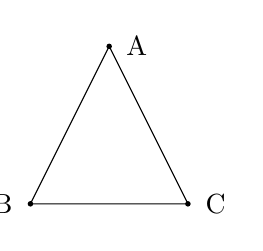
\begin{tikzpicture}
            \coordinate (A) at (2.0,3.0); 
            \coordinate (B) at (1.0,1.0);
            \coordinate (C) at (3.0,1.0);

            \draw (A) -- (B) -- (C) -- cycle;
            \fill (A) circle (1pt);
            \fill (B) circle (1pt);
            \fill (C) circle (1pt);

            \node at (A) {\hspace{2em}A};
            \node at (B) {\hspace{-2em}B};
            \node at (C) {\hspace{2em}C};
        \end{tikzpicture}
    \end{center}
\end{figure}

\subsection{Index Buffer}
(OpenGL: \cite{stage_gl_vertex_spec}; Direct3D: \cite{d3d_buffers})
Index Buffer sind ein Zusatz zu den Vertex Buffern und sie können genutzt werden, um den Speicherbedarf zu verringern. Sie ersetzen Vertex Buffer nicht, sondern arbeiten mit ihnen zusammen. Um Index Buffer nutzen zu können, muss immer ein Vertex Buffer existieren. 

In einem Index Buffer werden Indices eines Vertex Buffers gespeichert (zur Erinnerung: Vertex Buffer sind lediglich Arrays, jeder Vertex hat also einen festen Index). Wenn mit Hilfe eines Index Buffers gezeichnet wird, werden nicht alle Verticies eines Vertex Buffers gespeichert, sondern nur die Verticies, deren Indices im Index Buffer gespeichert sind.

Die Speichereinsparung entsteht dadurch, dass die selben Verticies mehrmals verwendet werden können, ohne dass die Vertex Daten mehrmals gespeichert werden müssen (denn es kann der selbe Index mehrmals im Index Buffer angegeben werden).

\subsection{Beispiel}

\begin{figure}
    \caption{Ein Viereck, bestehend aus zwei Dreiecken. Die beiden Zahlen kennzeichnen die jeweiligen Dreiecke.}
    \label{fig:vertexbufquad}
    \begin{center}
        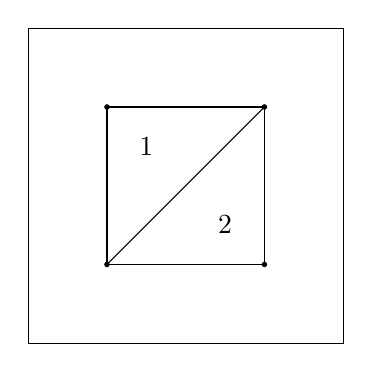
\begin{tikzpicture}
            \draw (1.0,3.0) -- (3.0,3.0) -- (3.0,1.0) -- (1.0,1.0) -- cycle;
            \draw (1.0,1.0) -- (3.0,3.0);
            \fill (1.0,3.0) circle (1pt);
            \fill (3.0,3.0) circle (1pt);
            \fill (3.0,1.0) circle (1pt);
            \fill (1.0,1.0) circle (1pt);
            \draw (0.0,0.0) rectangle (4.0,4.0);
            \node at (1.5,2.5) {1};
            \node at (2.5,1.5) {2};
        \end{tikzpicture}
    \end{center}
\end{figure}

Es soll das Viereck in Abbildung \ref{fig:vertexbufquad} gezeichnet werden. Wie üblich, wird ein Viereck aus zwei Dreiecken gezeichnet. Es kann direkt erkannt werden, dass die Verticies oben rechts und unten links für beide Dreiecke verwendet werden.

Würde man dieses Viereck ausschließlich mit einem Vertex Buffer zeichen, würde dieser wie folgt aussehen

$$
\left\{
\begin{tabular}{ccc}
    \{-0.75, -0.75\}, & \{0.75, 0.75\},  & \{-0.75, 0.75\}, \\
    \{-0.75, -0.75\}, & \{0.75, -0.75\}, & \{0.75, 0.75\}
\end{tabular}    
\right\}
$$
Offensichtlich werden die Vertex Daten $\{0.75, 0.75\}$ und $\{-0.75, -0.75\}$ doppelt gespeichert.
Dies ist in diesem Beispiel noch relativ harmlos, da für jeden Vertex nur die Positionsdaten gespeichert werden. Würden mit jedem Vertex allerdings noch mehr Daten assoziiert werden, müssten diese zusätzlichen Daten ebenfalls mehrfach gespeichert werden.

Diese Duplizierung der Daten lässt sich mit Hilfe von Index Buffern vermeiden. Wenn Index Buffer genutzt werden, würden die beiden Buffer aussehen wie folgt 

Vertex Buffer: %??? formatierung vertex buffer / index buffer überschrift
$$
\left\{
\begin{tabular}{ccc}
    \{-0.75, -0.75\}, & \{0.75, 0.75\}, & \{-0.75, 0.75\}, \\ 
                      & \{0.75, -0.75\} &
\end{tabular}    
\right\}
$$

Index Buffer:
$$
\left\{
\begin{tabular}{cccccc}
    0, & 1, & 2, & 0, & 3, & 1
\end{tabular}  
\right\}
$$
In diesem Beispiel ist die Speichereinsparung nur relativ gering, da nur zwei Verticies jeweils doppelt genutzt werden. In komplexeren Modellen, in denen Verticies deutlich öfter mehrfach genutzt werden, ist die Speichereinsparung allerdings dementsprechend größer. Ein Beispiel hierfür gibt Abbildung \ref{fig:vertexbufoct}, denn alle Verticies werden mehrfach verwendet. Vor allem der zentrale Vertex müsste in diesem Beispiel achtfach dupliziert werden.

\begin{figure}
    \caption{Eine Figur, bestehend aus acht Dreiecken.}
    \label{fig:vertexbufoct}
    \begin{center}
        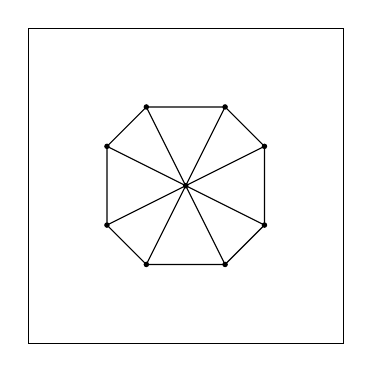
\begin{tikzpicture}
            \draw (1.5,3.0) -- (2.5,3.0) -- (3.0,2.5) -- (3.0,1.5) --
                  (2.5,1.0) -- (1.5,1.0) -- (1.0,1.5) -- (1.0,2.5) -- cycle;
            \draw (1.5,3.0) -- (2.5,1.0);
            \draw (2.5,3.0) -- (1.5,1.0);
            \draw (3.0,2.5) -- (1.0,1.5);
            \draw (3.0,1.5) -- (1.0,2.5);

            \fill (1.5,3.0) circle (1pt);
            \fill (2.5,3.0) circle (1pt);
            \fill (3.0,2.5) circle (1pt);
            \fill (3.0,1.5) circle (1pt);
            \fill (2.5,1.0) circle (1pt);
            \fill (1.5,1.0) circle (1pt);
            \fill (1.0,1.5) circle (1pt);
            \fill (1.0,2.5) circle (1pt);
            \fill (2.0,2.0) circle (1pt);

            \draw (0.0,0.0) rectangle (4.0,4.0);
        \end{tikzpicture}
    \end{center}
\end{figure}

Wenn Index Buffer genutzt werden, ist selbstverständlich nach wie vor die Reihenfolge, in der die Verticies an die GPU gegeben werden, wichtig. Die Reihenfolge wird nun allerdings durch die Reihenfolge der Indices im Index Buffer bestimmt, und nicht durch die Reihenfolge der Verticies im Vertex Buffer.

\subsection{Uniform Buffer}
Zusätzlich zu den Vertex und Index Buffern, die Daten pro Vertex bestimmen, existieren ebenfalls sogenannte Uniform Buffer, die Daten bereitstellen, die während eines Shader Pipeline durchlaufes konstant bleiben und auf die von allen Shadern aus zugegriffen werden kann.

Dies kann beispielsweise genutzt werden, wenn ein Objekt nur eine Farbe haben soll. Es wäre möglich, die Farbe durch den Vertex Buffer in die Pipeline zu geben. Diese Lösung wäre allerdings nicht gut, da dieselbe Farbe dann mit jedem Vertex erneut von der CPU zur GPU kopiert werden würde, was unnötig viel Bandbreite verbraucht, da die Farbe ja ohnehin immer dieselbe ist. Wenn stattdessen ein Uniform Buffer genutzt werden würde, würde der Wert nur ein einziges Mal kopiert werden. (OpenGL: \cite{gl_uniforms}; Direct3D: \cite{d3d_buffers})
